\section{Loi de commande} 
\subsection{Loi de contrôle et comportements} \label{sec:controle}
Afin d'étendre la stratégie bio-inspirée présentée précédemment au cas actif, nous considérons que les composantes perturbatrices $\delta \mathbf{I}$, en concret les scalaires axial $\delta I_{ax}$ et latéral $\delta I_{lat}$ présentés dans l'équation (\ref{eq:axial_lateral}).

La Table \ref{tab:proprietes} suggère d'appliquer la loi de contrôle suivante, d'après \cite{Boyer2013}: 

\begin{equation}
    v = C \quad ; \quad \omega = k \cdot \delta I_{lat}
\end{equation}
où $C$ est une constante positive qui permet au robot d'avancer vers l'avant, et $k$ est un gain pour contrôler la vitesse angulaire du robot poisson $\omega$. 

À partir de la Table \ref{tab:proprietes}, nous pouvons modifier le comportement dynamique du robot poisson: 
\begin{enumerate} [label=(\alph*), ref=(3.1.\alph*)]
    \item Si $k > 0$, cette loi de contrôle force \textbf{le capteur à être attiré par tout objet conducteur} et garantit que le capteur est repoussé par un objet isolant. \label{item:a}
    \begin{itemize}
        \item De ce fait, lorsqu'un objet conducteur conducteur se trouve à droite (ou à gauche, respectivement), le capteur se tourne vers la droite (ou la gauche, respectivement). Et lorsqu'un objet conducteur se trouve devant le capteur, le capteur avance sans changer d'orientation.
        \item En revanche, lorsqu'un objet isolant est situé à droite (ou à gauche, respectivement), cette loi de contrôle fait réagir le robot poisson comme s'il y avait un objet conducteur symétrique sur la gauche (ou sur la droite, respectivement).
    \end{itemize}
    \item \label{item:b} Si $k < 0$, cette loi force \textbf{le capteur à être attiré par tout objet isolant} et repoussé par les objets conducteurs. 
    \vspace{0.5cm}
    \item Si nous multiplions $k$ par le signe de $\delta I_{ax}$, nous obtenons les mêmes comportements pour des objets conducteurs ou isolants, ce qui assure au capteur, pour $k > 0$ d'être \textbf{attiré par tout objet}, et pour $k < 0$ d'être \textbf{repoussé par tout objet non transparent électriquement}. \label{item:c}
\end{enumerate}
\newpage
\subsection{Résultats obtenus}

Personnellement, le cas \ref{item:a} ne marche pas très bien, mais les cas \ref{item:b} et \ref{item:c} marchent bien. \vspace{0.2cm}

Pour le cas \ref{item:b}, où $k < 0$, nous pouvons voir dans la Figure \ref{fig:k_inferieur_0} comment le robot poisson est attiré par l'objet isolant, indépendemment de la position de ce dernier. 
Pour ce comportement, j'ai donné des poids différents aux tenseurs de polarisation en fonction de s'il s'agit d'un objet conducteur, isolant ou un mur :
\begin{lstlisting}[language=matlab, caption={Extrait du fichier \mcode{f_currents.m}}, firstnumber = 77, aboveskip=-0.6 \baselineskip, belowskip=-0.4 \baselineskip]
K = k_cond*0.9 - k_isol*0.9 + k_murs*0.6;
\end{lstlisting}

\begin{figure}[h!]
\centering
\begin{minipage}{0.45\textwidth}
  \centering
  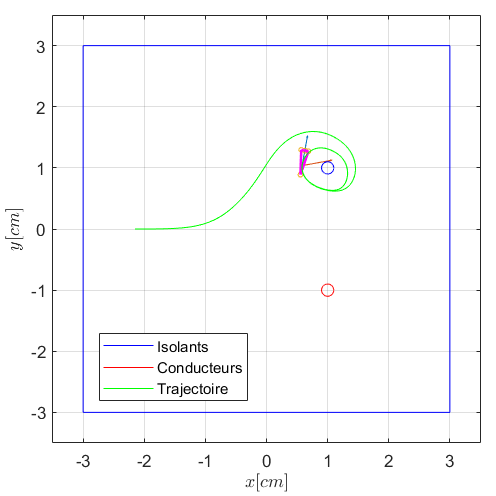
\includegraphics[width=\linewidth]{assets/essais/k_inferieur_0/k_inferieur_0.png}
\end{minipage}%
\begin{minipage}{0.45\textwidth}
  \centering
  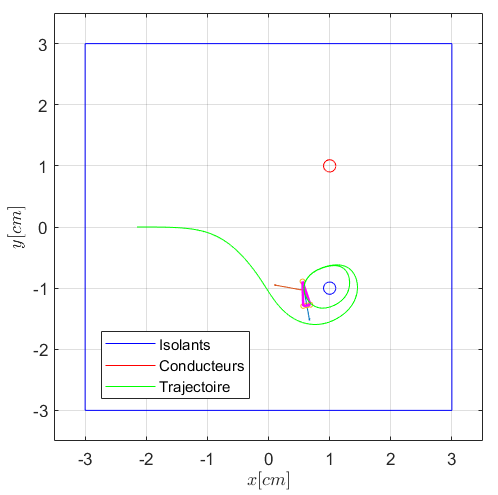
\includegraphics[width=\linewidth]{assets/essais/k_inferieur_0/k_inferieur_0_2.png}
\end{minipage}
\caption{\centering Robot poisson attiré par un conducteur isolant lorsque $k <0$ \ref{item:b}.}
\label{fig:k_inferieur_0}
\end{figure}

Pour le cas \ref{item:c}, nous observons dans la Figure comment le robot est repoussé par n'importe quel type d'objet, et comment les commandes reviennent et font le poisson tourner en cercles, tout en évitant les obstacles. Les poids choisis pour cette simulation sont les suivants: 
\begin{lstlisting}[language=matlab, caption={Extrait du fichier \mcode{f_currents.m}}, firstnumber = 77, aboveskip=-0.3 \baselineskip, belowskip=-0.6 \baselineskip]
K = k_cond*0.9 + k_isol*0.9 + k_murs*0.6;
\end{lstlisting}

\begin{figure}[h!]
\centering
\begin{minipage}{0.45\textwidth}
  \centering
  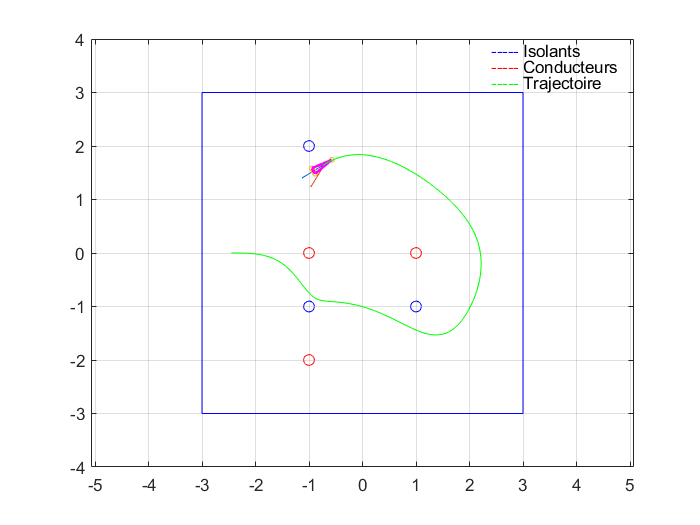
\includegraphics[width=\linewidth]{assets/essais/6_objets/6_objets.png}
\end{minipage}%
\begin{minipage}{0.45\textwidth}
  \centering
  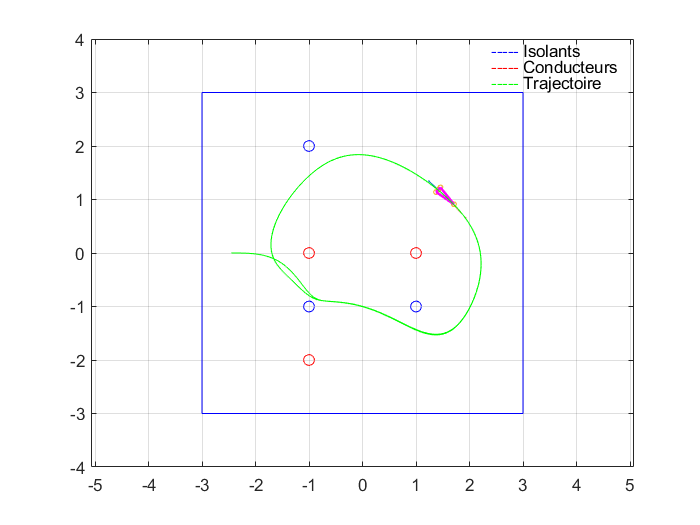
\includegraphics[width=\linewidth]{assets/essais/6_objets/6_objets_2.png}
\end{minipage}
\caption{\centering Robot poisson attiré par un conducteur isolant lorsque $k <0$ \ref{item:b}.}
\label{fig:k_inferieur_0}
\end{figure}